\documentclass[border=3pt,tikz]{standalone}
\usepackage{amsmath}
\usetikzlibrary{calc}
\usetikzlibrary{arrows.meta} % for arrow size
\begin{document}
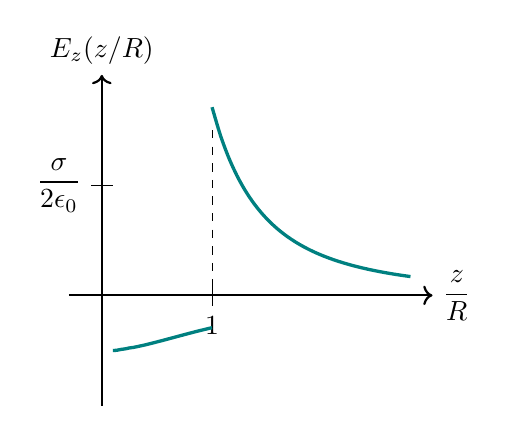
\begin{tikzpicture}[scale=1.4, rotate=0]
    \draw[thick, ->] (-0.3, 0) -- (3, 0) node [right] {$\dfrac{z}{R}$};
    \draw[thick, ->] (0, -1) -- (0, 2) node [above] {$E_z(z/R)$};
    \draw[] (1, 0.1)-- (1, -0.1) node [below] {$1$};
    \draw[] (0.1, 1.0) -- (-0.1, 1.0) node [left] {$\dfrac{\sigma}{2\epsilon_0}$};
    \draw[teal, very thick, domain=0.1:1, smooth, variable=\x,] plot ({\x}, {1/(\x *\x) * (1/sqrt(1+\x * \x)-1)});
    \draw[teal, very thick, domain=1:2.8, smooth, variable=\x,] plot ({\x}, {1/(\x *\x) * (1/sqrt(1+\x * \x)+1)});
    \draw[dashed] (1, 1.5) -- (1, 0);
  \end{tikzpicture}
\end{document}